\clearpage
\newpage
\mbox{~}
\clearpage
\newpage

\chapter{Introduction}
\label{cha:intro}
In 2018, the English Wikipedia has been visited 207.83 billions of times, a 4.73\% increase year by year.\footnote{\url{https://stats.wikimedia.org/v2/\#/en.wikipedia.org/reading/total-page-views/normal|bar|1-Year|~total}} This shows that Wikipedia is one of the key tools for enhancing people knowledge, due to the easily accessible free information. However, the unstructured nature of its content does not enable straightforward machine processing.
% For this reason, projects like Wikidata were created.
Wikidata\footnote{\url{https://www.wikidata.org/}} acts as central storage for structured data of its Wikimedia sister projects, including Wikipedia, Wikivoyage, Wikisource, and others.

Data quality is a crucial factor for the trustworthiness of Wikipedia and Wikidata content. In fact, Wikipedia provides mature citation guidelines to enforce high quality standard.\footnote{\url{https://en.wikipedia.org/wiki/Wikipedia:Citing_sources}}
Likewise, Wikidata allows to store references to (ideally authoritative) sources along with its data.

Nevertheless, \textbf{less than a quarter} of the Wikidata knowledge base (KB) statements currently has a reference to \textbf{non-wiki} sources, and roughly an \textbf{half} of them is totally \textbf{unreferenced}.\footnote{\url{https://docs.google.com/presentation/d/1XX-yzT98fglAfFkHoixOI1XC1uwrS6f0u1xjdZT9TYI/edit?usp=sharing}, slides 15 to 19}
The problem can be alleviated in several ways: we could encourage the community to focus on the referencing task. Another option could be the alignemnt of Wikidata entities to a set of external databases, which can be automated by software. This is a particularly interesting option because it provides a repeatable process.

\begin{figure}[t]
  \begin{center}
   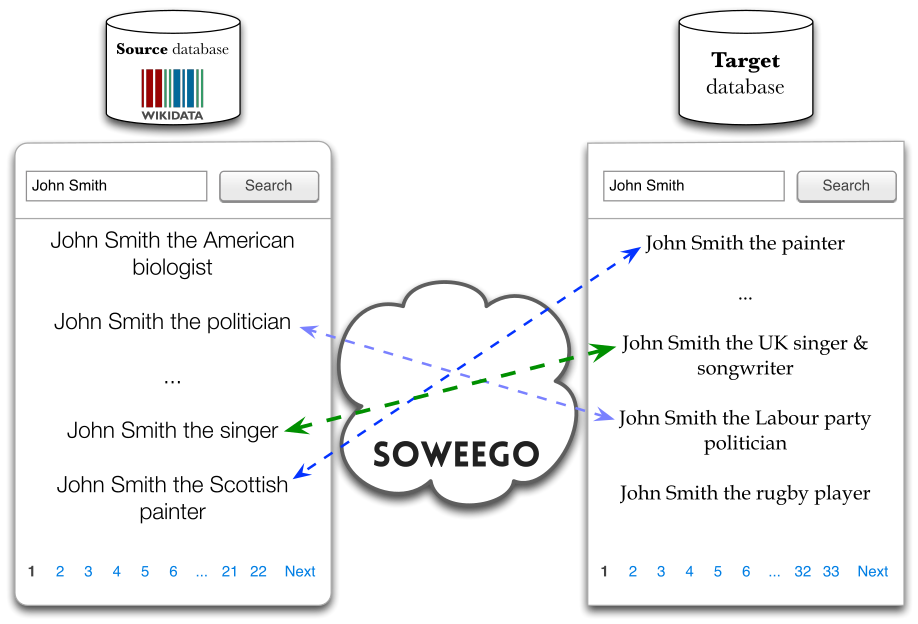
\includegraphics[height=200px]{images/matchexample.png}
   \captionof{figure}{\texttt{soweego} creates a connection (read performs disambiguation) between entries of the source database (Wikidata) and a target database. Image by \href{https://meta.wikimedia.org/wiki/User:Hjfocs}{\texttt{Hjfocs}}, \href{https://creativecommons.org/licenses/by-sa/4.0/deed.en}{CC BY-SA 4.0}}
   \label{fig:soweegomatch}
  \end{center}
\end{figure}

We define the problem as follows: given a Wikidata entity, find a suitable match in the target database.
This is not a trivial task, with homonyms being the first challenge.
For instance, suppose we would like to know more about the singer \textit{John Smith}.
We type the name into the Wikidata search box: multiple results appear, and it takes a while to find the person we are looking for.
Unfortunately, Wikidata does not hold much information about him and our search moves to another database, like MusicBrainz\footnote{\url{https://musicbrainz.org}}.
We must repeat the same procedure as with Wikidata, and after some digging, we manage to find John Smith the singer. This is a match: the MusicBrainz entity can be linked to Wikidata.
\texttt{soweego} aims at solving the issue at a large scale, via disambiguation of a source Wikidata entity to a target database entry. Figure~\ref{fig:soweegomatch} depicts the solution.

Wikidata entities are designed to store this kind of links. In particular, entities like John Smith are called \textit{items} and each of them is composed of an \textit{identifier}, a \textit{fingerprint}, and a set of \textit{statements}.\footnote{\url{https://www.mediawiki.org/wiki/Wikibase/DataModel/Primer}}
Each statement is broken down into \textit{claims} (i.e., property, value pairs) and optional \textit{references} (i.e., the sources of the factual information).
For instance, John Smith could have the claim (\texttt{given name}, \texttt{John}), together with its reference (\texttt{stated in}, \texttt{Duckburg Municipality archive}).
The identifier links to external sources are expressed as claims too.
The John Smith match between Wikidata and MusicBrainz would be e.g., expressed as a claim over the Wikidata item with identifier \texttt{Q666} (\texttt{MusicBrainz artist ID}, \texttt{77a1c579-3532-491c-86bd-595ddd4780cc}), where the latter value corresponds to the MusicBrainz identifier.

Officially, \texttt{soweego} has the following goals:\footnote{\url{https://meta.wikimedia.org/wiki/Grants:Project/Hjfocs/soweego\#Project_goals}}
\begin{enumerate}
    \item to ensure live maintenance of identifiers for people in Wikidata, via link validation;
    \item to develop a set of linking techniques that align people in Wikidata to corresponding identifiers in external catalogs;
    \item to ingest links into Wikidata, either through a bot (confident links), or mediated by curation (non-confident links);
    \item to achieve exhaustive coverage (ideally 100\%) of identifiers over 4 large-scale trusted catalogs;
    \item to deliver a self-sustainable application that can be easily operated by the community after the end of the project.
\end{enumerate}

The remainder of this thesis is structured as follows. In section \ref{cha:2} we report a brief review of the state of the art. The preliminary analysis of the candidate targets is detailed in section \ref{cha:3}. Section \ref{cha:4} describes the project architecture with a focus on the matching strategies, which we evaluate against MusicBrainz in section \ref{cha:5}. We draw our conclusions in section \ref{cha:conclusioni}.

